\chapter{Anexo 1: resultados experimentales}
\label{anexo1}

\section{Comparación parámetros $G$ y $N$}
A continuación se muestran los resultados de las pruebas que hemos realizados variando los parámetros $G$ y $N$ en los tres escenarios de prueba que disponíamos. En la \autoref{tab: comparativa de parámetros $G$ y $N$} se muestran la media de parámetros obtenidos tras realizar 25 experimentos sobre cada caso de prueba.
\begin{figure}[H]
	\begin{center}
		\centering
		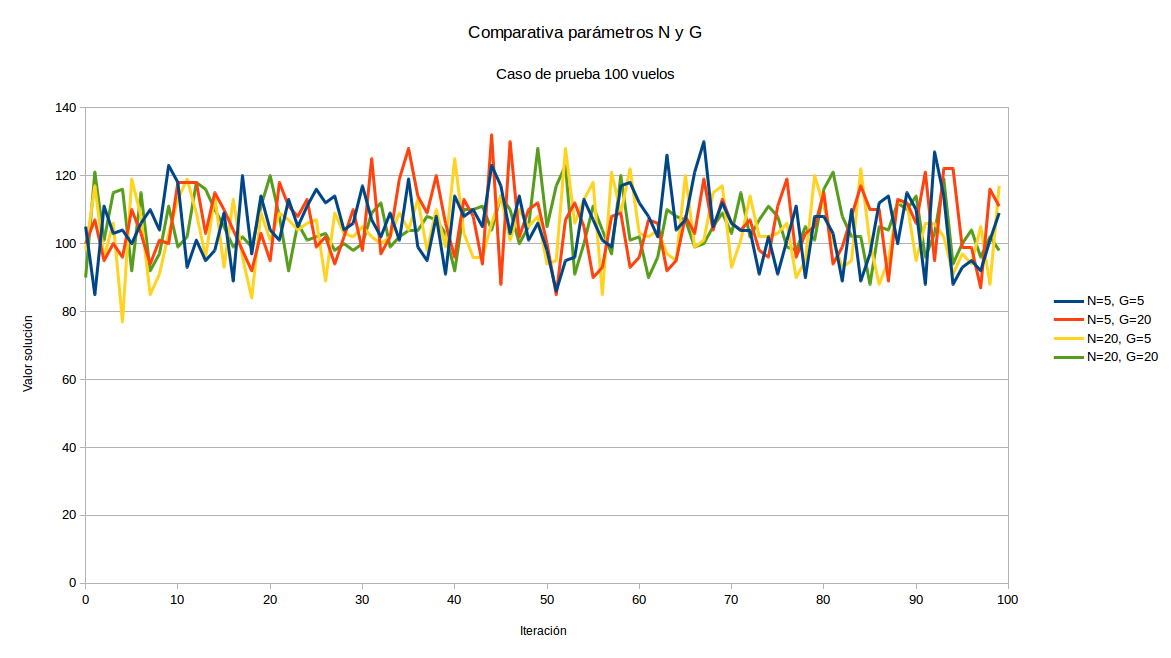
\includegraphics[width=1\textwidth]{./imagenes/heuristico/comparativa_parametros_100_vuelos.png}
		\caption{Evolución función objetivo con diferentes parámetros G y N}
		\label{fig: Evolución función objetivo con diferentes parámetros G y N}
	\end{center}
\end{figure}


\begin{table}[H]
	\centering
	\caption{Comparativa de parámetros $G$ y $N$}
	\label{tab: comparativa de parámetros $G$ y $N$}
	\begin{tabular}{|c|c|c|c|c|}
		\hline
		& \textbf{Problema A} & \textbf{Problema B} & \textbf{Problema C} & \textbf{Media porcentaje éxito} \\ \hline
		\textbf{N=2, G=10} & \% éxito: 64.1 & \% éxito: 94.2 &\% éxito: 99.5 & 85.93\% \\ \hline
		\textbf{N=2, G=30} & \% éxito: 65.2 & \% éxito: 95.1 &\% éxito: 99.5  & 86.60\%\\ \hline
		\textbf{N=2, G=50} & \% éxito: 66.1  & \% éxito: 95.6  &\% éxito: 99.6 & 87.10\%\\ \hline
		\textbf{N=5, G=10} & \% éxito: 65.2  & \% éxito: 94.3 &\% éxito: 99.4  &86.30\%\\ \hline
		\textbf{N=5, G=30} & \% éxito: 65.7  &\textcolor{blue}{\% éxito: 95.7 } &\% éxito: 99.8 &87.06\% \\ \hline
		\textbf{N=5, G=50} & \textcolor{blue}{\% éxito: 66.8} &\% éxito: 95.6  & \textcolor{blue}{\% éxito: 99.8}  &\textcolor{red}{87.40\%} \\ \hline
		\textbf{N=10, G=10} & \% éxito: 64.2  &\% éxito: 94.1  &\% éxito: 99.3  &85.86\% \\  \hline
		\textbf{N=10, G=30} & \% éxito: 65.2  &\% éxito: 95.1  &\% éxito: 99.5  &86.60\% \\ \hline
		\textbf{N=10, G=50} & \% éxito: 65.6  &\% éxito: 95.1  &\% éxito: 99.6  &86.76\% \\ \hline
	\end{tabular}	
\end{table}

Las características de las simulaciones corresponden a las siguientes:
\begin{itemize}
	\item Las pruebas se han realizado sobre los 3 problemas disponibles.
	\item En todos los experimentos se considera el peor escenario: la capacidad de los sectores está limitada a 1.
	\item Se realizan 100 iteraciones sobre cada experimento.
	\item El parámetro $G$
\end{itemize}

\section{Resultados simulación}
\subsection{Caso de pruebas A}
Se considera como el peor escenario, ya que tiene un gran número de vuelos con rutas idénticas, lo que implica que una vez saturado todas las trayectorias de un vuelo, el resto que son similares serán cancelados.
\subsubsection{20 vuelos}
Resultados del problema A con 20 vuelos:
\begin{longtable}{| p{.17\textwidth} | p{.17\textwidth} |  p{.17\textwidth} | p{.17\textwidth}  | p{.17\textwidth} | }
	
	\hline
	\textbf{Iteración} & \textbf{Valor de la función objetivo} &\textbf{\% Vuelos con solución} \\ \hline
	\textbf{0} &46  &100\%  \\ \hline
	\textbf{1} &46  &100\%  \\ \hline
	\textbf{2} &48  &100\%  \\ \hline
	\textbf{3} &47  &100\%  \\ \hline
	\textbf{4} &46  &100\%  \\ \hline
	\textbf{5} &48  &100\%  \\ \hline
	\textbf{6} &48  &100\%  \\ \hline
	\textbf{7} &47  &100\%  \\ \hline
	\textbf{8} &47  &100\%  \\ \hline
	\textbf{9} &46  &100\%  \\ \hline
	\textbf{10} &46  &100\%  \\ \hline
	\textbf{11} &46  &100\%  \\ \hline
	\textbf{12} &46  &100\%  \\ \hline
	\textbf{13} &48  &100\%  \\ \hline
	\textbf{14} &47  &100\%  \\ \hline
	\textbf{15} &47  &100\%  \\ \hline
	\textbf{16} &47  &100\%  \\ \hline
	\textbf{17} &45  &95\%  \\ \hline
	\textbf{18} &47  &100\%  \\ \hline
	\textbf{19} &47  &100\%  \\ \hline
	\textbf{20} &48  &100\%  \\ \hline
	\textbf{21} &45  &95\%  \\ \hline
	\textbf{22} &47  &100\%  \\ \hline
	\textbf{23} &47  &100\%  \\ \hline
	\textbf{24} &47  &100\%  \\ \hline
	\textbf{25} &48  &100\%  \\ \hline
				&Media: \textbf{46.8}  &Media: \textbf{99.61}\%  \\ \hline
	\caption{Resultados problema A 20 vuelos }
	\label{tab: Resultados problema A 20 vuelos}

\end{longtable}




\subsubsection{100 vuelos}
Resultados del problema A con 100 vuelos:
\begin{longtable}{| p{.17\textwidth} | p{.17\textwidth} |  p{.17\textwidth} | p{.17\textwidth}  | p{.17\textwidth} | }
	\hline
	\textbf{Iteración} & \textbf{Valor de la función objetivo} &\textbf{\% Vuelos con solución} \\ \hline
	\textbf{0} &124  &65\%  \\ \hline
	\textbf{1} &112  &61\%  \\ \hline
	\textbf{2} &120  &63\%  \\ \hline
	\textbf{3} &122  &64\%  \\ \hline
	\textbf{4} &122  &62\%  \\ \hline
	\textbf{5} &120  &60\%  \\ \hline
	\textbf{6} &114  &58\%  \\ \hline
	\textbf{7} &116  &62\%  \\ \hline
	\textbf{8} &127  &55\%  \\ \hline
	\textbf{9} &119  &61\%  \\ \hline
	\textbf{10} &121  &63\%  \\ \hline
	\textbf{11} &111  &57\%  \\ \hline
	\textbf{12} &115  &60\%  \\ \hline
	\textbf{13} &114  &58\%  \\ \hline
	\textbf{14} &121  &62\%  \\ \hline
	\textbf{15} &110  &60\%  \\ \hline
	\textbf{16} &119  &61\%  \\ \hline
	\textbf{17} &124  &65\%  \\ \hline
	\textbf{18} &118  &65\%  \\ \hline
	\textbf{19} &112  &60\%  \\ \hline
	\textbf{20} &112  &60\%  \\ \hline
	\textbf{21} &131  &68\%  \\ \hline
	\textbf{22} &116  &60\%  \\ \hline
	\textbf{23} &123  &64\%  \\ \hline
	\textbf{24} &121  &65\%  \\ \hline
	\textbf{25} &119  &61\%  \\ \hline
				&Media: \textbf{118.57}  &Media: \textbf{61.69}\%  \\ \hline

	\caption{Resultados problema A 100 vuelos } % needs to go inside longtable environment
	\label{tab: Resultados problema A 100 vuelos}

	
\end{longtable}





\section{Caso de pruebas B}
Se considera un escenario moderado, hay varios vuelos similares pero parten en momentos de tiempo muy distanciados entre sí, por lo que salvo en contadas ocasiones no habrá conflictos entre vuelos similares.
\subsubsection{20 vuelos}
Resultados del problema B con 20 vuelos:
\begin{longtable}{| p{.17\textwidth} | p{.17\textwidth} |  p{.17\textwidth} | p{.17\textwidth}  | p{.17\textwidth} | }
	\hline

		\textbf{Iteración} & \textbf{Valor de la función objetivo} &\textbf{\% Vuelos con solución} \\ \hline
		\textbf{0} &47  &100\%  \\ \hline
		\textbf{1} &47  &100\%  \\ \hline
		\textbf{2} &47  &100\%  \\ \hline
		\textbf{3} &47  &100\%  \\ \hline
		\textbf{4} &47  &100\%  \\ \hline
		\textbf{5} &47  &100\%  \\ \hline
		\textbf{6} &47  &100\%  \\ \hline
		\textbf{7} &47  &100\%  \\ \hline
		\textbf{8} &47  &100\%  \\ \hline
		\textbf{9} &47  &100\%  \\ \hline
		\textbf{10} &47  &100\%  \\ \hline
		\textbf{11} &47  &100\%  \\ \hline
		\textbf{12} &47  &100\%  \\ \hline
		\textbf{13} &47  &100\%  \\ \hline
		\textbf{14} &47  &100\%  \\ \hline
		\textbf{15} &47  &100\%  \\ \hline
		\textbf{16} &47  &100\%  \\ \hline
		\textbf{17} &47  &100\%  \\ \hline
		\textbf{18} &47  &100\%  \\ \hline
		\textbf{19} &47  &100\%  \\ \hline
		\textbf{20} &47  &100\%  \\ \hline
		\textbf{21} &47  &100\%  \\ \hline
		\textbf{22} &47  &100\%  \\ \hline
		\textbf{23} &47  &100\%  \\ \hline
		\textbf{24} &47  &100\%  \\ \hline
		\textbf{25} &47  &100\%  \\ \hline
					&Media: \textbf{47}  &Media: \textbf{100}\%  \\ \hline
	\caption{Resultados problema B 20 vuelos } % needs to go inside longtable environment
	\label{tab: Resultados problema B 20 vuelos}

	
\end{longtable}




\subsubsection{100 vuelos}
Resultados del problema B con 100 vuelos:
\begin{longtable}{| p{.17\textwidth} | p{.17\textwidth} |  p{.17\textwidth} | p{.17\textwidth}  | p{.17\textwidth} | }
	\hline
	\textbf{Iteración} & \textbf{Valor de la función objetivo} &\textbf{\% Vuelos con solución} \\ \hline
	\textbf{0} &200  &93\%  \\ \hline
	\textbf{1} &202  &96\%  \\ \hline
	\textbf{2} &204  &96\%  \\ \hline
	\textbf{3} &203  &96\%  \\ \hline
	\textbf{4} &203  &95\%  \\ \hline
	\textbf{5} &198  &93\%  \\ \hline
	\textbf{6} &201  &93\%  \\ \hline
	\textbf{7} &201  &94\%  \\ \hline
	\textbf{8} &197  &93\%  \\ \hline
	\textbf{9} &199  &92\%  \\ \hline
	\textbf{10} &199  &93\%  \\ \hline
	\textbf{11} &199  &93\%  \\ \hline
	\textbf{12} &200  &92\%  \\ \hline
	\textbf{13} &199  &93\%  \\ \hline
	\textbf{14} &198  &92\%  \\ \hline
	\textbf{15} &202  &94\%  \\ \hline
	\textbf{16} &205  &96\%  \\ \hline
	\textbf{17} &214  &96\%  \\ \hline
	\textbf{18} &199  &93\%  \\ \hline
	\textbf{19} &202  &96\%  \\ \hline
	\textbf{20} &200  &93\%  \\ \hline
	\textbf{21} &201  &93\%  \\ \hline
	\textbf{22} &200  &93\%  \\ \hline
	\textbf{23} &198  &92\%  \\ \hline
	\textbf{24} &200  &93\%  \\ \hline
	\textbf{25} &199  &93\%  \\ \hline
				&Media: \textbf{200.88}  &Media: \textbf{93.73}\%  \\ \hline
	\caption{Resultados problema B 100 vuelos } 
	\label{tab: Resultados problema B 100 vuelos}

	
\end{longtable}





\subsection{Caso de pruebas C}
Se consdera el escenario más favorable: vuelos muy diferentes entre sí, con un varias rutas alternativas y con varios aeropuertos de salida.
\subsubsection{20 vuelos}
Resultados del problema C con 20 vuelos:
\begin{longtable}{| p{.17\textwidth} | p{.17\textwidth} |  p{.17\textwidth} | p{.17\textwidth}  | p{.17\textwidth} | }
	\hline
	\textbf{Iteración} & \textbf{Valor de la función objetivo} &\textbf{\% Vuelos con solución} \\ \hline
	\textbf{0} &45 &100\%  \\ \hline
	\textbf{1} &45 &100\%  \\ \hline
	\textbf{2} &45 &100\%  \\ \hline
	\textbf{3} &45 &100\%  \\ \hline
	\textbf{4} &45 &100\%  \\ \hline
	\textbf{5} &45 &100\%  \\ \hline
	\textbf{6} &45 &100\%  \\ \hline
	\textbf{7} &45 &100\%  \\ \hline
	\textbf{8} &45 &100\%  \\ \hline
	\textbf{9} &45 &100\%  \\ \hline
	\textbf{10} &45 &100\%  \\ \hline
	\textbf{11} &45 &100\%  \\ \hline
	\textbf{12} &45 &100\%  \\ \hline
	\textbf{13} &45 &100\%  \\ \hline
	\textbf{14} &45 &100\%  \\ \hline
	\textbf{15} &45 &100\%  \\ \hline
	\textbf{16} &45 &100\%  \\ \hline
	\textbf{17} &45 &100\%  \\ \hline
	\textbf{18} &45 &100\%  \\ \hline
	\textbf{19} &45 &100\%  \\ \hline
	\textbf{20} &45 &100\%  \\ \hline
	\textbf{21} &45 &100\%  \\ \hline
	\textbf{22} &45 &100\%  \\ \hline
	\textbf{23} &45 &100\%  \\ \hline
	\textbf{24} &45 &100\%  \\ \hline
	\textbf{25} &45 &100\%  \\ \hline
				&Media: \textbf{45}  &Media: \textbf{100}\%  \\ \hline
	\caption{Resultados problema C 20 vuelos } % needs to go inside longtable environment
	\label{tab: Resultados problema C 20 vuelos}

	
\end{longtable}



\subsubsection{100 vuelos}

Resultados del problema C con 100 vuelos:
\begin{longtable}{| p{.17\textwidth} | p{.17\textwidth} |  p{.17\textwidth} | p{.17\textwidth}  | p{.17\textwidth} | }
	\hline
	\textbf{Iteración} & \textbf{Valor de la función objetivo} &\textbf{\% Vuelos con solución} \\ \hline
	\textbf{0} &218  &100\%  \\ \hline
	\textbf{1} &218  &100\%  \\ \hline
	\textbf{2} &218  &100\%  \\ \hline
	\textbf{3} &218  &100\%  \\ \hline
	\textbf{4} &218  &100\%  \\ \hline
	\textbf{5} &218  &100\%  \\ \hline
	\textbf{6} &218  &100\%  \\ \hline
	\textbf{7} &218  &100\%  \\ \hline
	\textbf{8} &218  &100\%  \\ \hline
	\textbf{9} &218  &100\%  \\ \hline
	\textbf{10} &218  &100\%  \\ \hline
	\textbf{11} &215  &99\%  \\ \hline
	\textbf{12} &218  &100\%  \\ \hline
	\textbf{13} &218  &100\%  \\ \hline
	\textbf{14} &218  &100\%  \\ \hline
	\textbf{15} &218  &100\%  \\ \hline
	\textbf{16} &218  &100\%  \\ \hline
	\textbf{17} &218  &100\%  \\ \hline
	\textbf{18} &218  &100\%  \\ \hline
	\textbf{19} &218  &100\%  \\ \hline
	\textbf{20} &218  &100\%  \\ \hline
	\textbf{21} &218  &100\%  \\ \hline
	\textbf{22} &218  &100\%  \\ \hline
	\textbf{23} &218  &100\%  \\ \hline
	\textbf{24} &218  &100\%  \\ \hline
	\textbf{25} &218  &100\%  \\ \hline
				&Media: \textbf{217.88}  &Media: \textbf{99.96}\%  \\ \hline
	\caption{Resultados problema C 100 vuelos } % needs to go inside longtable environment
	\label{tab: Resultados problema C 100 vuelos}

	
\end{longtable}




